%----------------------------------------------------------------------------------------
%    PACKAGES AND THEMES
%----------------------------------------------------------------------------------------

\documentclass[aspectratio=169,xcolor=dvipsnames]{beamer}
\usetheme{SimplePlus}

\usepackage{tikz}
\usepackage{hyperref}
\usepackage{graphicx} % Allows including images
\usepackage{booktabs} % Allows the use of \toprule, \midrule and \bottomrule in tables

%----------------------------------------------------------------------------------------
%    TITLE PAGE
%----------------------------------------------------------------------------------------

\title{Predictive Analytics in Healthcare}
\subtitle{HI 743}

\author{}

\institute
{
    Department of Health Informatics and Administration \\
    Zilber College of Public Health \\
    University of Wisconsin - Milwaukee% Your institution for the title page
}
\date{January 23, 2025} % Date, can be changed to a custom date

%----------------------------------------------------------------------------------------
%    PRESENTATION SLIDES
%----------------------------------------------------------------------------------------

\begin{document}

\begin{frame}
    % Print the title page as the first slide
    \titlepage
\end{frame}

\begin{frame}{Overview}
    % Throughout your presentation, if you choose to use \section{} and \subsection{} commands, these will automatically be printed on this slide as an overview of your presentation
    \tableofcontents
\end{frame}
%------------------------------------------------
\section{HI 743}
\begin{frame}{HI 743 - Predictive Analytics in Healthcare}
    \begin{itemize}
        \item \textbf{Instructor}: Ryan Gallagher
        \item \textbf{Time \& Place}: Thursdays 2:30PM - 5:00PM in EH 103
        \item \textbf{Textbooks}: \textit{Fundamentals of Machine Learning for Predictive Data Analytics: Algorithms, Worked Examples, and Case Studies} by John D. Kelleher, Brian Mac Namee and Aoife D' Arey
        \\
        \vspace{0.2cm}
        \textit{Introduction to Statistical Learning with Applications in R (Second Edition)} by Gareth James, Daniela Witten, Trevor Hastie, Robert Tibshirani \\(Freely Distributed at \texttt{statlearning.com})
        \item \textbf{Required Materials}: Textbook, A Computer (Laptop preferably), R (software), \& RStudio (IDE for R)
    \end{itemize}
\end{frame}

%------------------------------------------------
\section{Introductions}
\subsection{About Me}
% About Me
\begin{frame}{About Me}

    \begin{tikzpicture}[overlay, remember picture]
        \node at (2, -0.5) {
\includegraphics[width=3cm]{images/MCWLogo_green.png}}; % Replace with your image path
    \end{tikzpicture}

    \begin{tikzpicture}[overlay, remember picture]
        \node at (12.5, 0) {\includegraphics[width=3cm]{images/UW–Eau_Claire_seal.png}}; % Replace with your image path
    \end{tikzpicture}

    \begin{center}
        Ryan Gallagher \\
        \vspace{0.5cm}
        Biostatistician\\
        MCW/CW Advanced Genomics Lab \\
        \vspace{0.5cm}
        M.A. in Biostatistics \& Data Science (MCW) \\
        B.S. in Statistics \& Applied Physics, double major (UWEC)
    \end{center}
\end{frame}
%% What I do (Explain my role at MCW)
\begin{frame}{What I Do}
    \begin{itemize}
        \item Biostatistics
        \begin{itemize}
            \item Hypothesis Testing
            \item Model Fitting
            \item Differential Expression Analysis
        \end{itemize}
        \item Bioinformatics
        \begin{itemize}
            \item Pipeline Development
            \item Genomic Data Analysis
        \end{itemize}
        \item Programming
        \begin{itemize}
            \item R for Statistics
            \item Python for Data Processing Pipeline
            \item Bash for Linux Cluster
        \end{itemize}
    % Picture of Prom 
    \end{itemize}

    \begin{tikzpicture}[overlay, remember picture]
        \node at (13, 4) {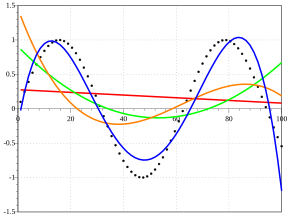
\includegraphics[width=3cm]{images/Curve_fitting.svg.png}}; % Replace with your image path
    \end{tikzpicture}

    \begin{tikzpicture}[overlay, remember picture]
        \node at (10, 3) {
\includegraphics[width=3cm]{images/R_logo.png}}; % Replace with your image path
    \end{tikzpicture}

    \begin{tikzpicture}[overlay, remember picture]
        \node at (13, 2) {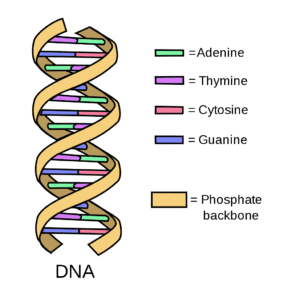
\includegraphics[width=3cm]{images/Stockphoto-DNA-Simple2-284x300.png}}; % Replace with your image path
    \end{tikzpicture}
\end{frame}

\begin{frame}{What I Do}
    I work on my lab's \textbf{Structural Variance Initiative}, which:
    \begin{enumerate}
        \item Recruits \& Consents Pediatrics Patients
        \item Sequences Entire Genome from Biological Sample
        \begin{enumerate}
            \item Oxford Nanopore Long-Read Sequencing 
            \item Bionano Optical Genome Mapping
        \end{enumerate}
        \item Processes Raw Sequencing Reads (Python + Bash)
        \begin{enumerate}
            \item Sequencing Data Management ($\sim1.5$TB)
            \item Raw Sequence Alignment + QC
            \item Identify SNPs + Small INDELs, CNVs, SVs
        \end{enumerate}
        \item Annotate Identified Variants
        \item Identify Potential Disease Causing Variants
    \end{enumerate}

    \begin{tikzpicture}[overlay, remember picture]
        \node at (12, 5) {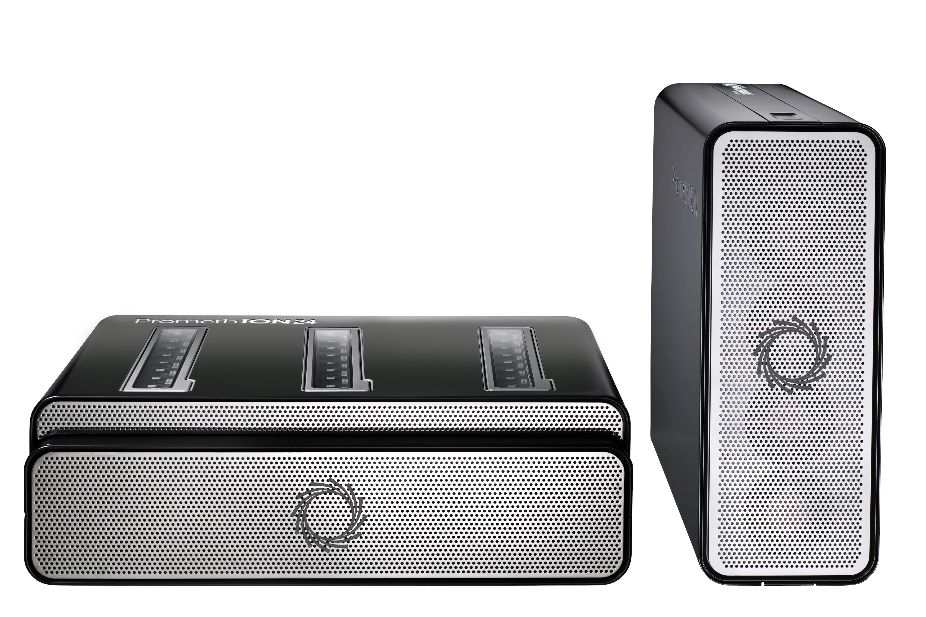
\includegraphics[width=3cm]{images/PromethION_P24_glamour_shot_form_word_doc_1.0.tif.png}}; % Replace with your image path
    \end{tikzpicture}

    \begin{tikzpicture}[overlay, remember picture]
        \node at (12, 2) {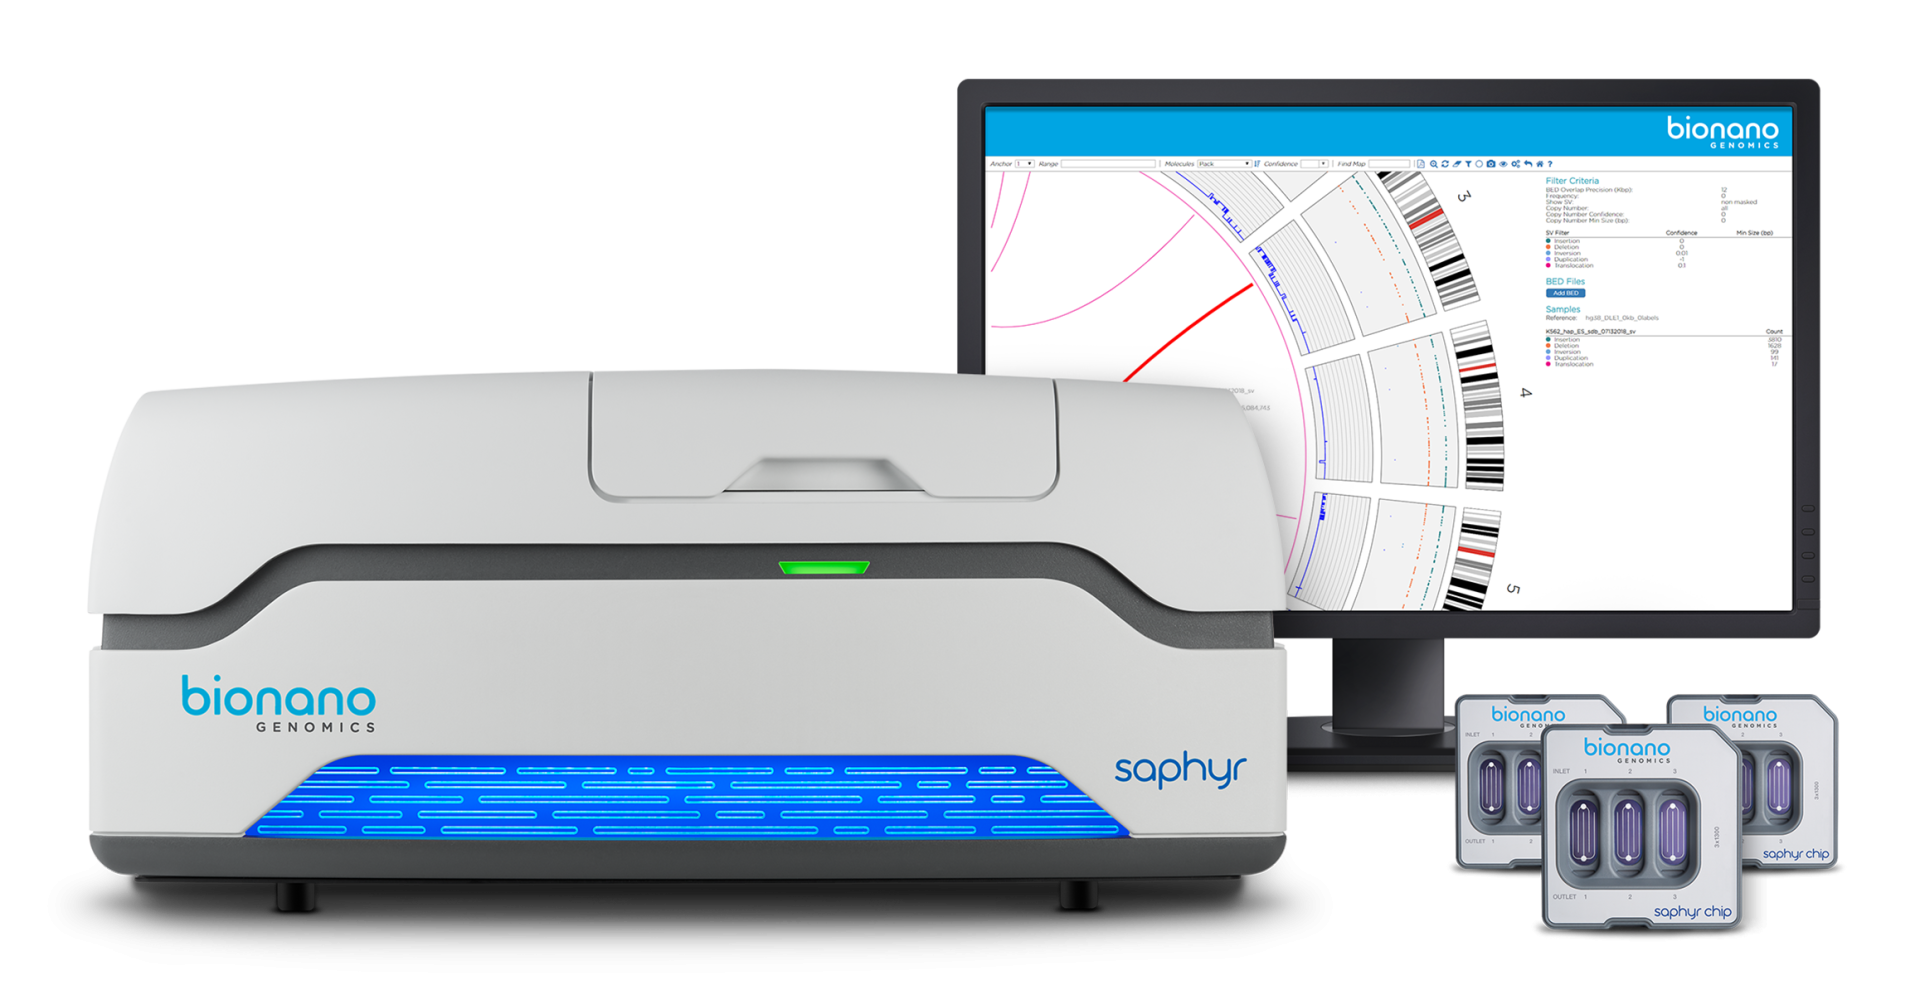
\includegraphics[width=3cm]{images/IMG_Bionano.png}}; % Replace with your image path
    \end{tikzpicture}
\end{frame}

\begin{frame}{What I Do}
        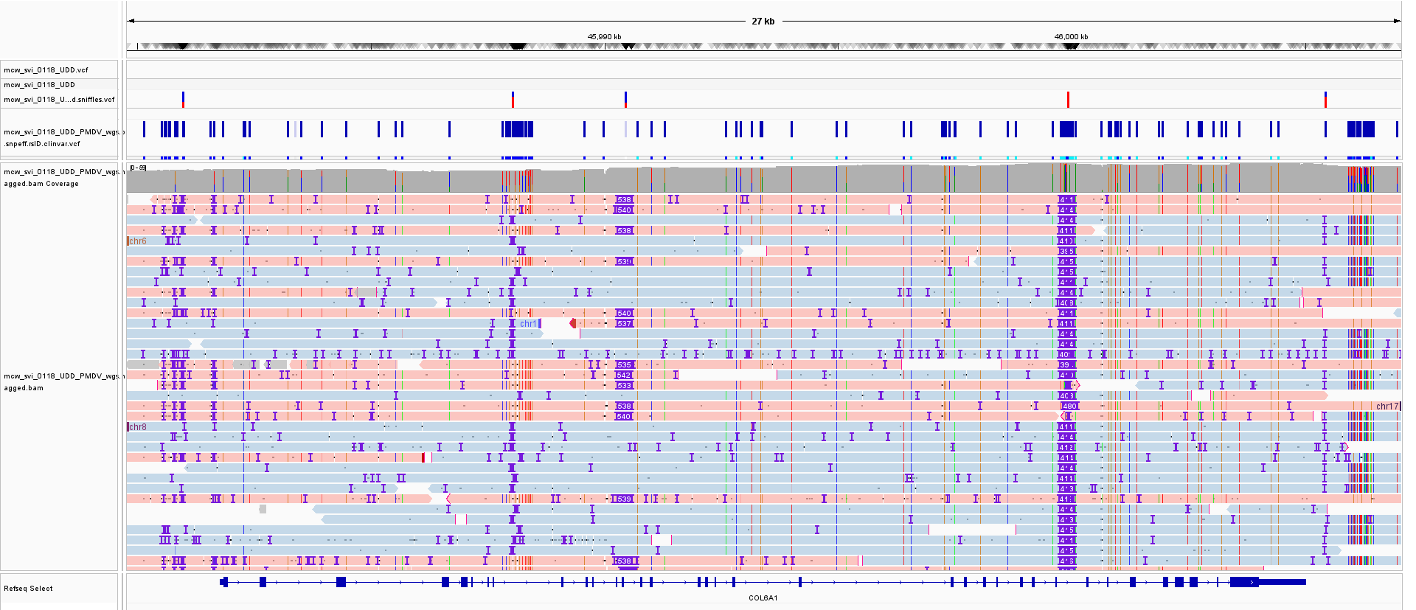
\includegraphics[scale=0.6]{images/IGV.png}
\end{frame}

\begin{frame}{What I Do}
        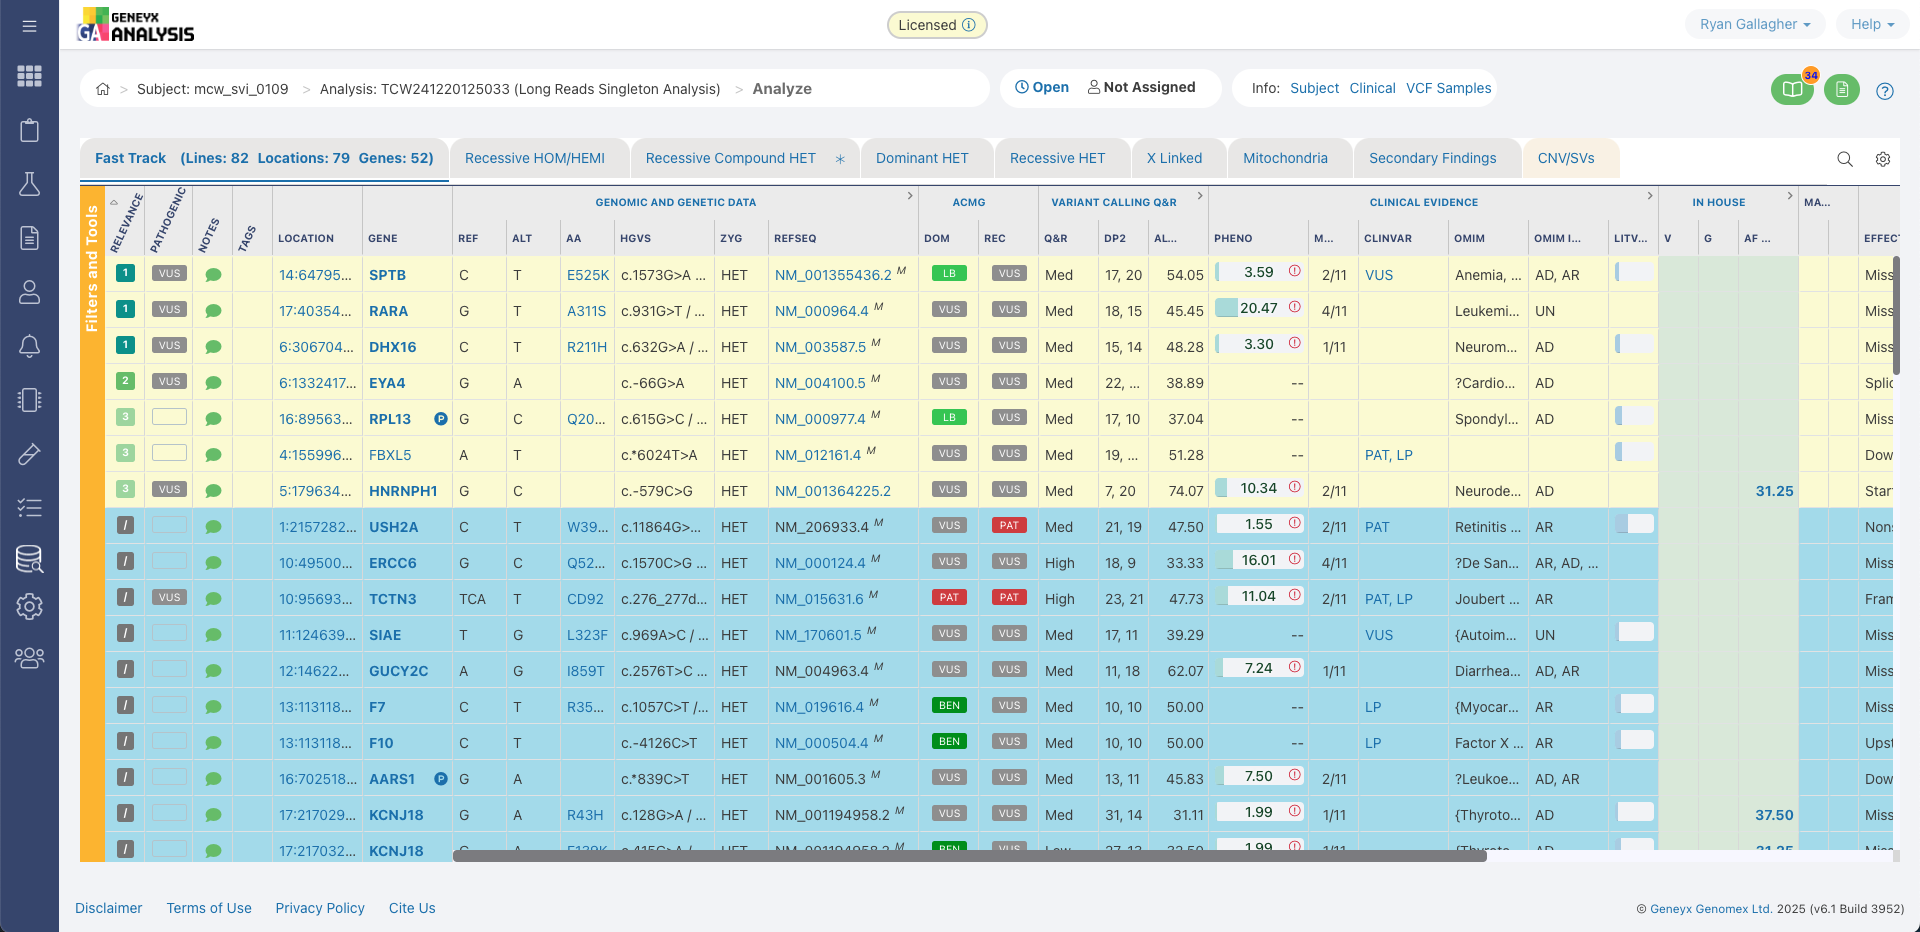
\includegraphics[scale=0.22]{images/geneyx.png}
\end{frame}

% Short Student Introductions (Gather Names)
\subsection{About You}
\begin{frame}{About You}
    \begin{center}
        [ Name ] \\
        {[ Program / Area of Focus ]} \\
        {[ Aspirations Post Education? ]} \\
        {[ Familiarity with Statistics? (Scale 1-10) ]} \\
        {[ Familiarity with Programming? (Scale 1-10) (Languages?) ]} \\
        {[ Do you have a Laptop? (Which OS?) ]}
    \end{center}
\end{frame}
% Small course motivation (why study analytics/ML)
%------------------------------------------------
%------------------------------------------------
\section{Syllabus}
\subsection{Syllabus Review}
\begin{frame}{Syllabus}
    \begin{center}
        Lets look at our syllabus
    \end{center}
\end{frame}

\subsection{Weekly Itinerary}
\begin{frame}{Week 2 - Course Motivations}
\textbf{Lecture:}
    \begin{itemize}
        \setlength{\itemsep}{.25cm}
        \item What is Predictive Data Analytics?
        \item What is Machine Learning? % Brief History in ISLR
        \item How does Machine Learning work?
        \item How is Machine Learning relevant to my field of interest?
    \end{itemize}
\end{frame}

\begin{frame}{Week 3 - Intro to R Language}
\textbf{Lecture:}
    \begin{itemize}
        \setlength{\itemsep}{.25cm}
        \item What is \texttt{R}?
        \item Why use \texttt{R}?
        \item Brief History of \texttt{R}
    \end{itemize}
\textbf{\texttt{R} Lab:}
    \begin{itemize}
        \setlength{\itemsep}{.25cm}
        \item Hands-on Tutorial in \textt{R}
        \item Data Manipulation with \textit{Tidyverse} Package
        \item \texttt{R} Figures
    \end{itemize}
\end{frame}

\begin{frame}{Week 4 - Data Exploration}
\textbf{Lecture:}
    \begin{itemize}
        \setlength{\itemsep}{.25cm}
        \item Data Quality
        \item Data Preparation
        \item Missing Values / Outliers
    \end{itemize}
\textbf{\texttt{R} Lab:}
    \begin{itemize}
        \item Hands-On Data Cleaning
        \item Data Visualization
    \end{itemize}
\end{frame}

\begin{frame}{Week 5 - Error Based Regression}
\textbf{Lecture:}
    \begin{itemize}
        \setlength{\itemsep}{.25cm}
        \item Simple Linear Regression
        \item Multiple Linear Regression \& Interpretation
        \item Nonlinear Regression \& Interpretation
    \end{itemize}
\textbf{\texttt{R} Lab:}
    \begin{itemize}
    \setlength{\itemsep}{.25cm}
        \item Multiple \& Nonlinear Regression
        \item Interpreting \texttt{R} Output
        \item Introduction to \texttt{RMarkdown} for Reporting
    \end{itemize}
\end{frame}

\begin{frame}{Week 6 - Classification / Logistic Regression}
\textbf{Lecture:}
    \begin{itemize}
        \setlength{\itemsep}{.25cm}
        \item Logistic Regression
        \item Generalized Linear Models
        \item Multinomial Logistic Regression
    \end{itemize}
\textbf{\texttt{R} Lab:}
    \begin{itemize}
    \setlength{\itemsep}{.25cm}
        \item Logistic Regression in \texttt{R}
        \item \texttt{glm()} function
    \end{itemize}
\end{frame}

\begin{frame}{Week 7 - Case Study (or Classification Continued)}
    \begin{center}
    
        This week will either be a continuation of the Classification methods. \\ 
        \vspace{1cm}
        Or \\
        \vspace{1cm}
        We will look at a case study which applies Classification methods to real-world data.
    \end{center}
\vspace{1cm}
\small\textbf{Project Idea is Due Following Week.}
\end{frame}

\begin{frame}{Week 8 - Information Based Learning}
\textbf{Lecture:}
    \begin{itemize}
        \setlength{\itemsep}{.25cm}
        \item Basics of Decision Trees
        \item Random Forest, Bagging, Boosting, etc..
        \item Tree "Pruning"
    \end{itemize}
\textbf{\texttt{R} Lab:}
    \begin{itemize}
    \setlength{\itemsep}{.25cm}
        \item Fitting Classification Trees
        \item Fitting Regression Trees
        \item Bagging Algorithms
    \end{itemize}
\end{frame}

\begin{frame}{Week 9 - SPRING BREAK!}
    \begin{center}
        \textbf{No Class!}
    \end{center}
\end{frame}

\begin{frame}{Week 10 - Unsupervised / Similarity-based Learning}
    \textbf{Lecture:}
    \begin{itemize}
        \setlength{\itemsep}{.25cm}
        \item Principal Component Analysis
        \item Clustering Methods
        \item Challenges of Unsupervised Learning
    \end{itemize}
\textbf{\texttt{R} Lab:}
    \begin{itemize}
    \setlength{\itemsep}{.25cm}
        \item K-Means Clustering
        \item PCA Example
    \end{itemize}
\end{frame}

\begin{frame}{Week 11 - Probability / Bayesian Methods in ML}
    \textbf{Lecture:}
    \begin{itemize}
        \setlength{\itemsep}{.25cm}
        \item Bayes' Thoerem
        \item Naive Bayes Model
        \item Probability Density Functions
    \end{itemize}
\textbf{\texttt{R} Lab:}
    \begin{itemize}
    \setlength{\itemsep}{.25cm}
        \item Naive Bayes Worked Examples
    \end{itemize}
\end{frame}

\begin{frame}{Week 12 - Neural Networks and Deep Learning}
    \textbf{Lecture:}
    \begin{itemize}
        \setlength{\itemsep}{.25cm}
        \item What is Deep Learning?
        \item Single Layer Neural Networks
        \item Multilayer Neural Networks
        \item Convolutional Neural Networks
    \end{itemize}
\textbf{\texttt{R} Lab:}
    \begin{itemize}
    \setlength{\itemsep}{.25cm}
        \item Single, Multi, and Convolutional Neural Networks Applied
    \end{itemize}
\end{frame}

\begin{frame}{Week 13 - Model Evaluation}
    \textbf{Lecture:}
    \begin{itemize}
        \setlength{\itemsep}{.25cm}
        \item Model Performance Measures
        \item Resampling Methods
        \item Cross Validation
    \end{itemize}
\textbf{\texttt{R} Lab:}
    \begin{itemize}
    \setlength{\itemsep}{.25cm}
        \item Validation Set Approach
        \item Cross-Validation
        \item Bootstrapping
    \end{itemize}
\end{frame}

\begin{frame}{Week 14 - Practical ML Application}
    \textbf{Lecture:}
    \begin{itemize}
        \setlength{\itemsep}{.25cm}
        \item When to use Machine Learning vs. Typical Methods
        \item Choosing a Machine Learning Approach
        \item Matching Approaches to Data
    \end{itemize}
\vspace{2cm}
\textbf{Lab portion will be dedicated to working on Final Project.}
\end{frame}

\begin{frame}{Week 15 - Work on Final Project}
\begin{center}
    \textbf{Classtime will be dedicated to working on Final Project.}\\
    \textbf{Project Due May 9th.}
\end{center}
\end{frame}

% Section by Section in Syllabus, just pull up PDF (take notes)
% Ideas for Labs / Github could be in here, maybe write own version 
%   of syllabus
%------------------------------------------------%------------------------------------------------
\section{CANVAS}
% Navigation
% Discussion Boards

%------------------------------------------------


%----------------------------------------------------------------------------------------

\end{document}